Completa la Tabla \ref{tab:resorte} considerando el alargamiento del resorte y el peso que se coloca.

\begin{multicols}{2}
    \begin{table}[H]
        \centering
        \caption{Datos sobre el alargamiento de un resorte debido al peso sostenido.}
        \label{tab:resorte}
        \begin{tabular}{|>{\columncolor{colorrds!80}\color{white}\bfseries}c|c|c|c|c|c|c|}
            \toprule
            Peso (kg)         & 0                    & $\frac{1}{2}$        & 1 & 2                    & 3                    & 5                     \\\cline{2-7}\midrule
            Alargamiento (cm) & \ifprintanswers 0\fi & \ifprintanswers 1\fi & 2 & \ifprintanswers 4\fi & \ifprintanswers 6\fi & \ifprintanswers 10\fi \\\cline{2-7}
            \bottomrule
        \end{tabular}
    \end{table}
    \begin{parts}
        \part ¿Qué tipo de relación funcional existe entre el alargamiento del resorte y el peso que se coloca?

        \begin{solutionbox}{1.5cm}
            Es una relación de variación proporcional.
        \end{solutionbox}

        \part ¿En qué punto de la gráfica la línea interseca al eje vertical?

        \begin{solutionbox}{1.5cm}
            En el punto (0, 0).
        \end{solutionbox}

        \part Dibuja en el plano cartesiano de la Figura \ref{fig:20230320205645_a} los puntos que corresponden
        al alargamiento del resorte y el peso que se le coloca, y únelos con una
        línea.

        \begin{figure}[H]
            \centering
            \ifprintanswers
                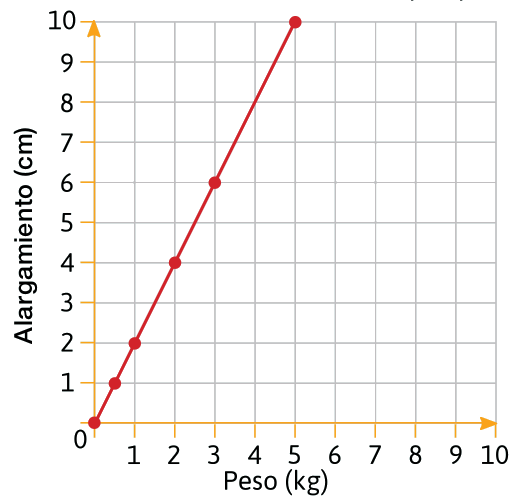
\includegraphics[width=.7\linewidth]{../images/20230320215503}
            \else
                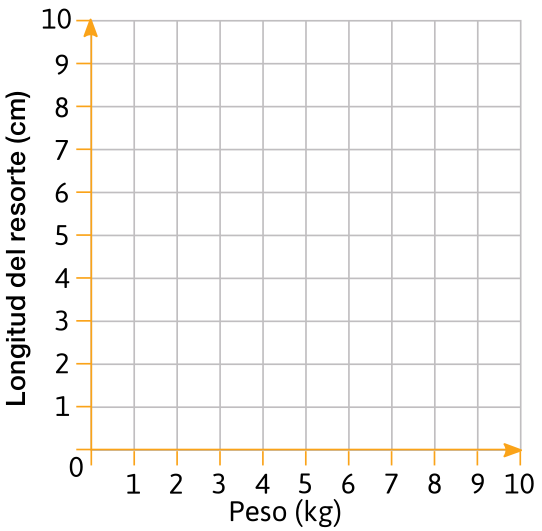
\includegraphics[width=.7\linewidth]{../images/20230320205645}
            \fi
            \caption{Plano cartesiano}
            \label{fig:20230320205645_a}
        \end{figure}


        % \begin{minipage}[t][5cm][b]{0.3\textwidth}

        % \columnbreak
        % ¿En qué se parecen y en qué difieren las dos gráficas de esta actividad?

        % \begin{solutionbox}{1.6cm}
        %     Ambas gráficas son líneas rectas; pero sólo la segunda interseca al
        %     eje vertical en el origen.
        % \end{solutionbox}
    \end{parts}
\end{multicols}